% !TEX root = ../root.tex
\section{Stability and Safety}
~\label{sec:safety}
% We begin by introducing the control theory foundation that provides the desired control closed-loop properties under possible uncertainties.
We begin by introducing the control-theoretic foundations that provide the desired closed-loop properties of stability and constraint satisfaction. We first review these concepts in the nominal setting, in which the dynamics are known exactly, and then extend the discussion to robust and stochastic formulations that explicitly account for uncertainty. The latter settings are particularly relevant in learning-based control, where the dynamics are only approximately known from data and the resulting model error must be incorporated into the analysis either as a bounded disturbance or as a probabilistic uncertainty description. \edits{\autoref{fig:stability_safety} illustrates the main concepts of this section.}

\begin{figure*}[t]
	\centering
	\begin{subfigure}[b]{0.32\textwidth}
		\centering
		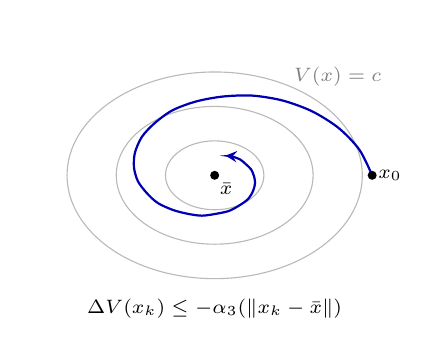
\begin{tikzpicture}[scale=1.25, >=stealth]
			\foreach \r in {0.5,1.0,1.5} {\draw[gray!55, thin] (0,0) ellipse ({\r} and {0.7*\r});}
			\node[gray, font=\scriptsize] at (1.25,1.0) {$V(x)=c$};
			\draw[thick, blue!70!black, ->] plot[smooth] coordinates {(1.60,0.00) (1.47,0.26) (1.26,0.48) (0.99,0.65) (0.69,0.76) (0.38,0.81) (0.08,0.80) (-0.19,0.75) (-0.43,0.66) (-0.61,0.53) (-0.74,0.39) (-0.81,0.23) (-0.82,0.08) (-0.78,-0.06) (-0.69,-0.18) (-0.58,-0.28) (-0.43,-0.35) (-0.28,-0.39) (-0.13,-0.41) (0.02,-0.39) (0.15,-0.36) (0.26,-0.30) (0.34,-0.24) (0.39,-0.16) (0.41,-0.08) (0.40,-0.01) (0.37,0.06) (0.32,0.11) (0.26,0.16) (0.18,0.19) (0.11,0.20)};
			\fill (0,0) circle (1.3pt);
			\node[font=\scriptsize, below right, inner sep=1pt] at (0.02,-0.05) {$\bar x$};
			\fill (1.6,0) circle (1.3pt);
			\node[font=\scriptsize, right, inner sep=2pt] at (1.6,0) {$x_0$};
			\node[font=\scriptsize] at (0,-1.35) {$\Delta V(x_k) \le -\alpha_3(\|x_k-\bar x\|)$};
			\path (-1.9,-1.5) rectangle (1.9,1.5);
		\end{tikzpicture}
		\caption{\edits{Nominal stability}}
		\label{fig:ss_nominal}
	\end{subfigure}%
	\begin{subfigure}[b]{0.32\textwidth}
		\centering
		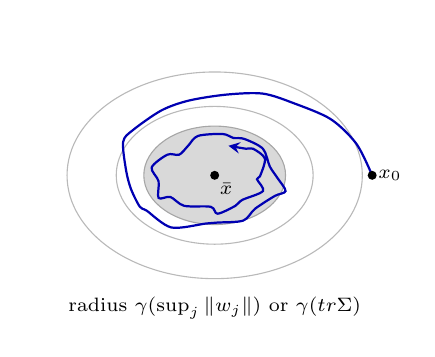
\begin{tikzpicture}[scale=1.25, >=stealth]
			\foreach \r in {1.0,1.5} {\draw[gray!55, thin] (0,0) ellipse ({\r} and {0.7*\r});}
			\fill[gray!30] (0,0) ellipse (0.72 and 0.5);
			\draw[gray!70, thin] (0,0) ellipse (0.72 and 0.5);
			\draw[thick, blue!70!black, ->] plot[smooth] coordinates {(1.60,0.00) (1.44,0.32) (1.18,0.57) (0.81,0.73) (0.49,0.83) (0.12,0.82) (-0.26,0.76) (-0.54,0.66) (-0.83,0.46) (-0.93,0.34) (-0.90,0.05) (-0.85,-0.14) (-0.76,-0.32) (-0.69,-0.36) (-0.44,-0.53) (-0.09,-0.49) (0.03,-0.48) (0.29,-0.46) (0.41,-0.34) (0.61,-0.21) (0.72,-0.16) (0.64,-0.03) (0.56,0.09) (0.49,0.27) (0.30,0.37) (0.19,0.38) (0.08,0.42) (-0.17,0.40) (-0.27,0.30) (-0.36,0.21) (-0.48,0.21) (-0.64,0.08) (-0.57,-0.06) (-0.57,-0.23) (-0.45,-0.22) (-0.31,-0.31) (-0.04,-0.32) (0.03,-0.39) (0.21,-0.31) (0.28,-0.25) (0.49,-0.16) (0.43,-0.04) (0.46,-0.01) (0.51,0.17) (0.39,0.27) (0.32,0.27) (0.14,0.30)};
			\fill (0,0) circle (1.3pt);
			\node[font=\scriptsize, below right, inner sep=1pt] at (0.02,-0.05) {$\bar x$};
			\fill (1.6,0) circle (1.3pt);
			\node[font=\scriptsize, right, inner sep=2pt] at (1.6,0) {$x_0$};
			\node[font=\scriptsize] at (0,-1.35) {radius $\gamma(\sup_j\|w_j\|)$ or $\gamma(\operatorname{tr}\Sigma)$};
			\path (-1.9,-1.5) rectangle (1.9,1.5);
		\end{tikzpicture}
		\caption{\edits{Robust and stochastic stability}}
		\label{fig:ss_robust}
	\end{subfigure}%
	\begin{subfigure}[b]{0.32\textwidth}
		\centering
		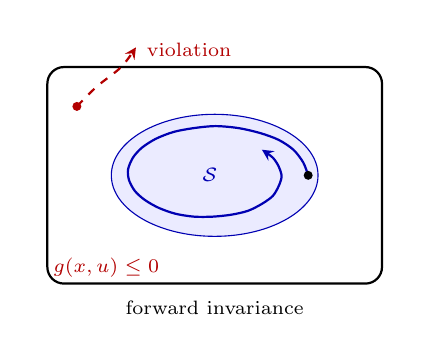
\begin{tikzpicture}[scale=1.25, >=stealth]
			\draw[thick, rounded corners=6pt] (-1.7,-1.1) rectangle (1.7,1.1);
			\node[font=\scriptsize, red!70!black, above right, inner sep=2pt] at (-1.7,-1.1) {$g(x,u)\le 0$};
			\fill[blue!8] (0,0) ellipse (1.05 and 0.62);
			\draw[blue!70!black, thin] (0,0) ellipse (1.05 and 0.62);
			\node[font=\scriptsize, blue!70!black] at (-0.05,0) {$\mathcal S$};
			\draw[thick, blue!70!black, ->] plot[smooth] coordinates {(0.95,0.00) (0.90,0.13) (0.80,0.26) (0.65,0.36) (0.46,0.43) (0.24,0.48) (0.01,0.50) (-0.21,0.48) (-0.42,0.44) (-0.60,0.37) (-0.74,0.28) (-0.83,0.18) (-0.88,0.06) (-0.87,-0.05) (-0.81,-0.16) (-0.71,-0.25) (-0.57,-0.33) (-0.40,-0.39) (-0.21,-0.42) (-0.02,-0.42) (0.17,-0.40) (0.34,-0.36) (0.48,-0.29) (0.59,-0.21) (0.65,-0.11) (0.68,-0.01) (0.65,0.09) (0.59,0.18) (0.48,0.26)};
			\fill (0.95,0) circle (1.3pt);
			\fill[red!70!black] (-1.4,0.7) circle (1.3pt);
			\draw[thick, red!70!black, dashed, ->] plot[smooth] coordinates {(-1.4,0.7) (-1.2,0.9) (-0.95,1.1) (-0.8,1.3)};
			\node[font=\scriptsize, red!70!black, right, inner sep=2pt] at (-0.75,1.28) {violation};
			\node[font=\scriptsize] at (0,-1.35) {forward invariance};
			\path (-1.9,-1.5) rectangle (1.9,1.5);
		\end{tikzpicture}
		\caption{\edits{Invariance and safety}}
		\label{fig:ss_invariance}
	\end{subfigure}\\[0.8em]
	\begin{subfigure}[b]{0.32\textwidth}
		\centering
		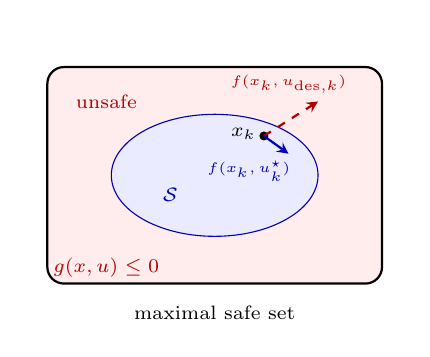
\begin{tikzpicture}[scale=1.25, >=stealth]
			\begin{scope}
				\clip[rounded corners=6pt] (-1.7,-1.1) rectangle (1.7,1.1);
				\fill[red!7] (-1.7,-1.1) rectangle (1.7,1.1);
				\fill[blue!8] (0,0) ellipse (1.05 and 0.62);
			\end{scope}
			\draw[thick, rounded corners=6pt] (-1.7,-1.1) rectangle (1.7,1.1);
			\node[font=\scriptsize, red!70!black, above right, inner sep=2pt] at (-1.7,-1.1) {$g(x,u)\le 0$};
			\draw[blue!70!black, thin] (0,0) ellipse (1.05 and 0.62);
			\node[font=\scriptsize, blue!70!black] at (-0.45,-0.2) {$\mathcal S$};
			\node[font=\scriptsize, red!70!black] at (-1.1,0.75) {unsafe};
			\node[font=\scriptsize] at (0,-1.4) {maximal safe set};
			\fill (0.5,0.4) circle (1.3pt);
			\node[font=\scriptsize, left, inner sep=2pt] at (0.48,0.42) {$x_k$};
			\draw[thick, red!70!black, dashed, ->] (0.5,0.4) -- (1.05,0.75);
			\node[font=\tiny, red!70!black, above, inner sep=1pt] at (0.75,0.8) {$f(x_k,u_{\mathrm{des},k})$};
			\draw[thick, blue!70!black, ->] (0.5,0.4) -- (0.75,0.22);
			\node[font=\tiny, blue!70!black, below left, inner sep=1pt] at (0.8,0.18) {$f(x_k,u_k^\star)$};
			\path (-1.9,-1.5) rectangle (1.9,1.5);
		\end{tikzpicture}
		\caption{\edits{Hamilton-Jacobi reachability}}
		\label{fig:ss_hj}
	\end{subfigure}%
	\begin{subfigure}[b]{0.32\textwidth}
		\centering
		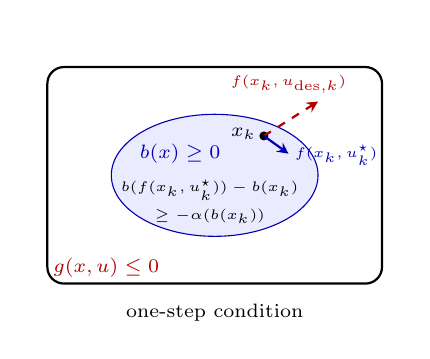
\begin{tikzpicture}[scale=1.25, >=stealth]
			\draw[thick, rounded corners=6pt] (-1.7,-1.1) rectangle (1.7,1.1);
			\node[font=\scriptsize, red!70!black, above right, inner sep=2pt] at (-1.7,-1.1) {$g(x,u)\le 0$};
			\fill[blue!8] (0,0) ellipse (1.05 and 0.62);
			\draw[blue!70!black, thin] (0,0) ellipse (1.05 and 0.62);
			\node[font=\scriptsize, blue!70!black] at (-0.35,0.22) {$b(x)\ge0$};
			\node[font=\tiny, align=center] at (-0.05,-0.27) {$b(f(x_k,u_k^\star)) - b(x_k)$\\[2pt]$\ge -\alpha(b(x_k))$};
			\node[font=\scriptsize] at (0,-1.4) {one-step condition};
			\fill (0.5,0.4) circle (1.3pt);
			\node[font=\scriptsize, left, inner sep=2pt] at (0.48,0.42) {$x_k$};
			\draw[thick, red!70!black, dashed, ->] (0.5,0.4) -- (1.05,0.75);
			\node[font=\tiny, red!70!black, above, inner sep=1pt] at (0.75,0.8) {$f(x_k,u_{\mathrm{des},k})$};
			\draw[thick, blue!70!black, ->] (0.5,0.4) -- (0.75,0.22);
			\node[font=\tiny, blue!70!black, right, inner sep=1pt] at (0.78,0.2) {$f(x_k,u_k^\star)$};
			\path (-1.9,-1.5) rectangle (1.9,1.5);
		\end{tikzpicture}
		\caption{\edits{Control barrier function}}
		\label{fig:ss_cbf}
	\end{subfigure}%
	\begin{subfigure}[b]{0.32\textwidth}
		\centering
		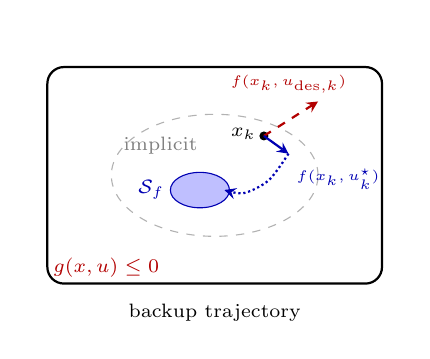
\begin{tikzpicture}[scale=1.25, >=stealth]
			\draw[thick, rounded corners=6pt] (-1.7,-1.1) rectangle (1.7,1.1);
			\node[font=\scriptsize, red!70!black, above right, inner sep=2pt] at (-1.7,-1.1) {$g(x,u)\le 0$};
			\draw[gray!60, dashed, thin] (0,0) ellipse (1.05 and 0.62);
			\node[font=\scriptsize, gray] at (-0.55,0.3) {implicit};
			\fill[blue!25] (-0.15,-0.15) ellipse (0.3 and 0.18);
			\draw[blue!70!black, thin] (-0.15,-0.15) ellipse (0.3 and 0.18);
			\node[font=\scriptsize, blue!70!black, left, inner sep=2pt] at (-0.45,-0.15) {$\mathcal S_f$};
			\node[font=\scriptsize] at (0,-1.4) {backup trajectory};
			\fill (0.5,0.4) circle (1.3pt);
			\node[font=\scriptsize, left, inner sep=2pt] at (0.48,0.42) {$x_k$};
			\draw[thick, red!70!black, dashed, ->] (0.5,0.4) -- (1.05,0.75);
			\node[font=\tiny, red!70!black, above, inner sep=1pt] at (0.75,0.8) {$f(x_k,u_{\mathrm{des},k})$};
			\draw[thick, blue!70!black, ->] (0.5,0.4) -- (0.75,0.22);
			\node[font=\tiny, blue!70!black, below right, inner sep=1pt] at (0.8,0.1) {$f(x_k,u_k^\star)$};
			\draw[blue!70!black, densely dotted, thick, ->] plot[smooth] coordinates {(0.75,0.22) (0.55,-0.05) (0.3,-0.18) (0.1,-0.15)};
			\path (-1.9,-1.5) rectangle (1.9,1.5);
		\end{tikzpicture}
		\caption{\edits{Predictive safety filter}}
		\label{fig:ss_psf}
	\end{subfigure}
	\caption{\edits{Illustration of the stability and safety notions of this section. (a) Nominal stability: a Lyapunov function $V$ decreases along closed-loop trajectories (level sets in gray) and the state converges to the equilibrium $\bar x$. (b) Robust and stochastic stability: under disturbances $w$, the state converges to a neighbourhood of $\bar x$ (shaded), whose size depends on the disturbance bound or the noise covariance. (c) Safety: constraint satisfaction at one time instant does not imply safety (red dashed); safety is guaranteed by an invariant set $\mathcal S$ contained in the constraints. (d)--(f) Safety filters: the desired input $u_{\mathrm{des},k}$ would leave the safe set and is modified to $u_k^\star$. HJ reachability computes the maximal safe set $\mathcal S$ offline and its complement (red) contains the states from which a constraint violation cannot be avoided. A CBF certifies invariance of $\{b(x)\ge0\}$ by the one-step condition on $b(x_{k+1})$. A PSF does not compute the safe set (dashed) but certifies safety by a backup trajectory (dotted) into a smaller terminal set $\mathcal S_f$. }}
	\label{fig:stability_safety}
\end{figure*}


We first recall the standard comparison function classes used throughout this section~\cite{khalil2002nonlinear}. A function $\alpha : \mathbb{R}_{\ge 0} \to \mathbb{R}_{\ge 0}$ is of class $\mathcal{K}$ if it is continuous, strictly increasing, and satisfies $\alpha(0)=0$. It is of class $\mathcal{K}_\infty$ if additionally $\alpha(r)\to\infty$ as $r\to\infty$. A function $\beta : \mathbb{R}_{\ge0}\times\mathbb{R}_{\ge0}\to\mathbb{R}_{\ge0}$ is of class $\mathcal{KL}$ if $\beta(\cdot,s)\in\mathcal K$ for each fixed $s$, and $\beta(r,s)\to0$ as $s\to\infty$ for each fixed $r$.

\subsection{\texorpdfstring{\edits{Nominal Stability}}{Nominal Stability}}
Stability concerns the asymptotic behaviour of a system around an equilibrium. Throughout this section, unless otherwise stated, the properties considered are local, i.e., they hold in a neighbourhood of the equilibrium.
When the dynamics $f$ are known, stability concerns an equilibrium $\bar x$ of system~\eqref{eq:system} in closed loop with a policy $u_k=\pi(x_k)$.

\begin{defn}[Nominal stability~\cite{khalil2002nonlinear}]\label{def:lyapunov}
	Let $\bar x$ be an equilibrium of system~\eqref{eq:system} under the
	policy $u_k=\pi(x_k)$ and with $w_k \equiv 0$. The equilibrium $\bar x$ is
	\begin{itemize}
		\item stable if there exist $\gamma \in \mathcal K$ and $r > 0$ such that
		      \[
			      \|x_k - \bar x\|
			      \le
			      \gamma(\|x_0 - \bar x\|)
		      \]
		      for all $ k \ge 0$ and all initial conditions satisfying $\|x_0 - \bar x\| < r$;
		\item asymptotically stable if there exist $\beta\in\mathcal{KL}$ and $r > 0$ such that
		      \[
			      \|x_k-\bar x\|
			      \le
			      \beta(\|x_0-\bar x\|,k)
		      \]
		      for all $k \ge 0$ and all initial conditions satisfying  $\|x_0 - \bar x\| < r$.
	\end{itemize}
\end{defn}

Lyapunov's direct method certifies stability through a pointwise decrease condition on a scalar energy-like function.

\begin{thm}[Lyapunov's direct method~\cite{khalil2002nonlinear}]\label{thm:lyapunov}
	Let $\bar x$ be an equilibrium and $\mathcal{D}$ a neighbourhood of
	$\bar x$. Suppose there exists a function
	$V : \mathcal{D} \to \mathbb{R}$ satisfying
	\[
		\alpha_1(\|x-\bar x\|)
		\le
		V(x)
		\le
		\alpha_2(\|x-\bar x\|)
	\]
	for some $\alpha_1,\alpha_2\in\mathcal K_\infty$, and let
	\[
		\Delta V(x_k)
		:=
		V(x_{k+1})-V(x_k)
	\]
	denote its one-step change along the closed-loop trajectories. Then:
	\begin{enumerate}
		\item if $\Delta V(x_k)\le0$ on $\mathcal D$, then $\bar x$ is stable;
		\item if there exists $\alpha_3\in\mathcal K_\infty$ such that
		      \[
			      \Delta V(x_k)
			      \le
			      -\alpha_3(\|x_k-\bar x\|)
		      \]
		      on $\mathcal D$, then $\bar x$ is asymptotically stable.
	\end{enumerate}
\end{thm}

\subsection{\texorpdfstring{\edits{Robust Stability}}{Robust Stability}}
In practice, however, the dynamics model used for control design is rarely exact. Learning-based controllers rely on models identified from finite data and therefore inevitably incur approximation error. This motivates robust stability notions that explicitly account for uncertainty and disturbances.

In the robust setting, the disturbance is assumed bounded, i.e., $w\in\mathcal{W}$, with $\mathcal{W}\subset \mathbb{R}^{n_\mathrm{w}}$ a compact set.
\edits{In the following, the model error and external disturbances are collected in the disturbance term $w$ of~\eqref{eq:system}. A commonly used robust stability notion is then \ac{ISS}, which characterizes the effect of the disturbance on the state trajectory.}

\begin{defn}[Input-to-state stability~\cite{khalil2002nonlinear}]\label{def:iss}
	Let $\bar x$ be an equilibrium of the system with $w \equiv \{0\}$, and consider
	\eqref{eq:system} in closed loop with $u_k = \pi(x_k)$ and disturbance
	sequence $w = \{w_k\}$, $w_k\in\mathcal{W}$. The closed-loop system is input-to-state stable
	if there exist $\beta \in \mathcal{KL}$ and $\gamma \in \mathcal{K}$
	such that, for every initial state $x_0$ and every bounded disturbance
	sequence~$w$,
	\begin{equation*}
		\|x_k - \bar x\|
		\le
		\beta(\|x_0 - \bar x\|,\, k)
		+
		\gamma\:\:\Big(\sup_{0 \le j < k} \|w_j\|\Big),
		\qquad k \ge 0 .
		\vspace{0.5em}
	\end{equation*}
\end{defn}

The ISS property separates the influence of the initial condition from that of the disturbance. The first term decays with time, whereas the second quantifies the residual error induced by uncertainty. % In learning-based control, the disturbance term often represents the mismatch between the learned model and the true dynamics.
%
As in the nominal case, ISS admits a Lyapunov characterization.

\begin{thm}[ISS-Lyapunov function~\cite{khalil2002nonlinear}]\label{thm:iss}
	Suppose there exists a function $V$ and
	$\alpha_1, \alpha_2 \in \mathcal{K}_\infty$ with
	\[
		\alpha_1(\|x - \bar x\|)
		\le
		V(x)
		\le
		\alpha_2(\|x - \bar x\|),
	\]
	whose one-step change along the closed-loop trajectories satisfies
	\begin{equation*}
		V(x_{k+1}) - V(x_k)
		\le
		-\alpha_3(\|x_k - \bar x\|)
		+
		\sigma(\|w_k\|)
	\end{equation*}
	for some $\alpha_3 \in \mathcal{K}_\infty$ and $\sigma \in \mathcal{K}$.
	Then the closed-loop system is input-to-state stable in the sense of~\autoref{def:iss}.
\end{thm}

When $w = \{0\}$, the ISS property reduces to
\[
	\|x_k - \bar x\|
	\le
	\beta(\|x_0 - \bar x\|, k),
\]
thus recovering the asymptotic stability of the nominal system. %When instead the disturbance is bounded, $\|w_k\| \le \bar w$, the gain term remains bounded and the closed loop converges to a neighbourhood of the equilibrium whose size depends on~$\bar w$.

A related robustness notion is incremental stability~\cite{angeli2002lyapunov}, which studies the convergence between pairs of trajectories rather than toward a single equilibrium. \edits{This concept extends to \ac{dISS}. Such properties can be used in order to compare nominal and perturbed trajectories in the presence of model mismatch.}

\subsection{\texorpdfstring{\edits{Stochastic Stability}}{Stochastic Stability}}
When the disturbance $w_k$ in~\eqref{eq:system} is modelled probabilistically, with $w_k \sim P_w$, the closed-loop system becomes a stochastic process. In this setting, stability is commonly formulated either in probability or in expectation.

\begin{defn}[Stochastic stability~\cite{mcallister2023stochastic,chatterjee2015stability}]\label{def:stochstab}
	Let $\bar x$ be an equilibrium for the system with $w \equiv \{0\}$, and consider~\eqref{eq:system} in closed loop with $u_k = \pi(x_k)$ and \ac{iid}, zero-mean disturbance $w_k \sim P_w$ with covariance $\Sigma$ and finite second moment. The equilibrium $\bar x$ is
	\begin{itemize}
		\item mean-square bounded if
		      \[
			      \limsup_{k \to \infty}\:\:
			      \mathbb{E}\,\|x_k - \bar x\|^2 < \infty .
		      \]
		\item robustly asymptotically stable in expectation if there exist $\beta \in \mathcal{KL}$ and $\gamma \in \mathcal{K}$ such that
		      \[
			      \mathbb{E}\,\|x_k - \bar x\|
			      \le \beta(\|x_0 - \bar x\|,\,k) + \gamma(\operatorname{tr}\Sigma),
			      \quad \forall k \geq 0.
		      \]
		\item asymptotically stable in expectation if it is robustly asymptotically stable in expectation with $\gamma \equiv 0$, i.e., there exists  $\beta \in \mathcal{KL}$ such that
		      \[
			      \mathbb{E}\,\|x_k - \bar x\|
			      \le \beta(\|x_0 - \bar x\|,\,k),
			      \quad \forall k \geq 0.
		      \]
	\end{itemize}
\end{defn}

%Probabilistic uncertainty descriptions arise naturally in Bayesian models like  Gaussian processes, where uncertainty is represented through a distribution rather than deterministic bounds.

As in the deterministic setting, stochastic stability can be established through a Lyapunov function satisfying an expected decrease condition.

\begin{thm}[Stochastic Lyapunov function~\cite{mcallister2023stochastic,chatterjee2015stability}]\label{thm:stochstab}
	Suppose there exist a function $V$ and
	$\alpha_1, \alpha_2 \in \mathcal{K}_\infty$ with
	\[
		\alpha_1(\|x - \bar x\|)
		\le
		V(x)
		\le
		\alpha_2(\|x - \bar x\|),
	\]
	a positive-definite stage cost $\ell$, and a constant
	$c \ge 0$ such that
	\begin{equation}
    \label{eq:lyap_dec_stoc}
		\mathbb{E}\!\left[V(x_{k+1}) \mid x_k\right] - V(x_k)
		\le
		-\ell(x_k) + c .
	\end{equation}
	Then, the closed loop is mean-square bounded and satisfies
	\begin{equation*}
		\limsup_{N \to \infty}
		\frac{1}{N}
		\sum_{k=0}^{N-1}
		\mathbb{E}\,\ell(x_k)
		\le c ,
	\end{equation*}
	and the equilibrium $\bar x$ is robustly asymptotically stable in expectation.
	If moreover $c = 0$, the equilibrium $\bar x$ is asymptotically stable in expectation.
\end{thm}

The constant $c$ in~\eqref{eq:lyap_dec_stoc} measures the residual effect of stochastic uncertainty and plays a role analogous to the disturbance gain in ISS. When $c = 0$ there is no residual stochastic term and $\bar{x}$ is recovered as an asymptotically stable equilibrium in expectation. Otherwise, the state remains bounded in mean square within a neighbourhood of $\bar x$, while the long-term average performance remains bounded by~$c$.

\subsection{\texorpdfstring{\edits{Invariance and Safety Filters}}{Invariance and Safety Filters}}
While stability concerns convergence toward equilibria, safety concerns the satisfaction of state and input constraints~\eqref{eq:constraints} over time.
\edits{Note that constraint satisfaction at a single time instant does not guarantee constraint satisfaction at future times, since there exist states satisfying the constraints from which a future constraint violation cannot be avoided under the system dynamics.} Safety therefore requires identifying sets from which the constraints remain satisfied for all future times. The central notion underlying safety (in terms of constraint satisfaction) is thus invariance.

\begin{defn}[Forward invariance~\cite{blanchini1999invariance}]
	Consider system~\eqref{eq:system} in closed loop with the policy $u_k=\pi(x_k)$, and let $\mathcal S \subseteq \mathbb R^{n_\mathrm{x}}$. The set $\mathcal S$ is said to be forward invariant if, for all initial conditions $x_0 \in \mathcal S$, the corresponding trajectory satisfies $x_k \in \mathcal S$ for all $k \ge 0$.
\end{defn}

A forward invariant set guarantees that trajectories initialized within it remain inside for all future times; safety then follows whenever such a set lies within the constraints. When the input is a decision variable, the relevant notion is control invariance, i.e., for every $x\in \mathcal S$, the existence of an input $u$ satisfying~\eqref{eq:constraints} and keeping the state in~$\mathcal S$.

Invariant sets can either be integrated directly as constraints in the control problem, as e.g., common practice in \ac{MPC}, \edits{or can be used to define a safety filter.} Safety filters are independent of the control policy and merely verify the safety of a proposed control action, and otherwise implement a safety-ensuring modification. We focus on the safety filter formulation in the following. For a tutorial overview of common safety filter formulations and their data-driven extensions, see also e.g., \cite{wabersich2023data}.

Classical approaches to safety characterize invariant sets through reachability analysis. In particular, \ac{HJ} reachability methods~\cite{bansal2017hamilton} compute the set of states from which trajectories can be kept within the constraints under the system dynamics by propagating backward the set of constraint-violating states. Such methods provide a global characterization of safety and typically yield tight approximations of the safe set under the assumed dynamics. However, their computational complexity scales poorly with the dimension of the state space, which limits their applicability to high-dimensional systems and has motivated various approximate
and learning-based extensions~\cite{wabersich2023data,8263977,mochen2018hamilton}.

An alternative approach relies on \acp{CBF}~\cite{ames2019control}, which enforce safety locally online through tractable conditions on the closed-loop dynamics. Analogously to Lyapunov functions for stability, barrier functions certify safety through conditions that guarantee forward invariance of a safe set. Consider a safe set of the form
\[
	\mathcal S := \{x \in \mathbb R^n : b(x)\ge0\},
\]
where $b : \mathbb R^n \to \mathbb R$. In discrete time, given a valid \ac{CBF}, one can  impose conditions on the control input such that
\[
	b(f(x_k,u_k)) - b(x_k)
	\ge
	-\alpha(b(x_k))
\]
for some $\alpha \in \mathcal K$ satisfying $\alpha(r) \le r$ for all $r \ge 0$. This condition ensures that trajectories cannot leave the safe set~$\mathcal S$, thereby rendering the set forward invariant. \edits{In discrete time, the barrier condition directly provides a one-step-ahead safety filter.} %, in which a nominal input proposed by a learning-based policy is modified only when necessary to ensure that the successor state satisfies the safety constraints. 
A common optimization problem is given by
\[
	\begin{aligned}
		u_k^\star
		:=
		\arg\min_{u_k}
		\quad              &
		\|u_k-u_{\mathrm{des},k}\|^2 \\
		\mathrm{s.t.}\quad &
		b(f(x_k,u_k)) - b(x_k)
		\ge
		-\alpha(b(x_k)),             \\
		                   &
		g(x_k,u_k)\leq 0 ,
	\end{aligned}
\]
where $u_{\mathrm{des},k}$ denotes the desired input generated by the nominal controller or learned policy at time $k$.

% \notes{{\bf [AC]:} we could replace $u_{des}$ with $\pi(x_k)$. Any preference?}

\edits{When comparing the computational cost of the two approaches, the construction of the safety certificate has to be distinguished from its online use. HJ reachability computes the value function on a grid over the state space. This is expensive and scales exponentially with the state dimension, but yields the (approximate) maximal safe set. A CBF only requires a function $b$ satisfying the barrier condition, which is cheaper to obtain but generally provides an inner approximation of the safe set \edits{and is in general difficult to construct for nonlinear systems.} Once the certificate is available, both filters are cheap to evaluate online, since the HJ value function can be used in the same way as a barrier function~\cite{borquez2024safety}.}

\edits{\Acp{PSF}~\cite{wabersich2018linear, wabersich2021predictive} do not require the construction of a large safe set, but enforce safety by means of finite-horizon trajectory planning.} Rather than explicitly computing a global invariant set, PSFs certify safety by ensuring the existence of a feasible backup trajectory that steers the system to a local invariant set.
Given the current state and a desired input proposed by a controller or learning-based policy, a \ac{PSF} solves a constrained finite-horizon optimal control problem of the form
\[
	\begin{aligned}
		\min_{\{u_{i|k}\}}
		\quad              &
		\|u_{0|k}-u_{\mathrm{des},k}\|^2                                     \\
		\mathrm{s.t.}\quad &
		x_{0|k}=x_k,                                                         \\
		                   &
		x_{i+1|k}=f(x_{i|k},u_{i|k}),  \quad \forall i \in \{0,\ldots,T-1\}, \\
		                   &
		g(x_{i|k},u_{i|k}) \leq 0, \quad \forall i \in \{0,\ldots,T-1\},     \\
		                   & x_{T|k}\in\mathcal S_f ,
	\end{aligned}
\]
where $T$ is the horizon and $\mathcal S_f$ denotes a terminal safe set for which safety can be guaranteed beyond the prediction horizon through a local controller. \edits{Here, $x_{i|k}$ and $u_{i|k}$ denote the state and input predicted $i$ steps ahead of time $k$, with $x_{0|k}=x_k$.}

The filter applies the first input $u_{0|k}^\star$ of the optimal sequence: whenever the desired input admits a feasible backup trajectory, it is passed through unmodified; otherwise, it is minimally adjusted. \edits{Recursive feasibility and closed-loop constraint satisfaction are guaranteed, provided that the terminal set $\mathcal S_f$ is (control) invariant.} \edits{In contrast to HJ reachability and CBFs, the safe set is not computed explicitly. The terminal set $\mathcal S_f$ can be small and simple, e.g., an invariant set of a local linear controller, and the region from which safety is certified is enlarged by the online planning over the horizon $T$. The computational effort is thereby shifted from the offline set computation to the online optimization.}

A closely related approach is shielding~\cite{alshiekh2018safe, bastani2021safe}, originally proposed in the context of \ac{RL}, in which a supervisory mechanism overrides the learned policy whenever it would lead to unsafe behaviour. In particular, model predictive shielding can be interpreted as a simulation-based variant of the \ac{PSF}: rather than solving an optimal control problem online, it forward-simulates a fixed backup policy and verifies that from the successor state there exists a feasible trajectory under the backup policy that ensures future constraint satisfaction. If this is not the case, the backup policy is applied instead.

% Conceptually, HJ reachability, CBFs, and \acp{PSF} differ primarily in how safety and invariance are represented and enforced. HJ methods compute global safe sets explicitly, CBFs enforce invariance locally through barrier certificates, and \acp{PSF} enforce safety implicitly through feasible receding-horizon trajectories. These approaches therefore exhibit complementary trade-offs between computational complexity, scalability, and conservativeness.
\edits{The three approaches thus differ with respect to the representation of the safe set: it is computed explicitly by HJ reachability, characterized by a barrier function in the case of a CBF, and defined implicitly by the existence of a feasible backup trajectory in the case of a \ac{PSF}.}

\edits{The complexity of the online problem differs between the approaches. For HJ reachability, the filter only requires the evaluation of the precomputed value function~\cite{borquez2024safety}. The CBF filter has a single one-step constraint. It is convex if $b\circ f$ is concave and $g$ is convex in $u_k$, e.g., for linear dynamics and a concave barrier function, and a small nonconvex program otherwise. In continuous time and for control-affine dynamics, the barrier constraint is affine in the input and the filter is a \ac{QP}~\cite{ames2019control}. The PSF is a finite-horizon optimal control problem with $T$ stages. It is a \ac{QP} for linear dynamics with polytopic constraints and terminal set, and a nonconvex nonlinear program for nonlinear dynamics.}

\subsection{\texorpdfstring{\edits{Robust and Stochastic Invariance}}{Robust and Stochastic Invariance}}
\edits{The notion of invariance extends to uncertain systems,} where it must hold for all admissible disturbances in robust settings~\cite{blanchini1999invariance}, and in probability or in expectation in stochastic ones~\cite{kofman2012probabilistic,hewing2018correspondence}.

In the robust case, \ac{HJ} reachability extends to worst-case analysis by computing invariant sets under adversarial disturbances~\cite{choi2023forward,seo2022real}, robust \acp{CBF} incorporate the uncertainty directly into the barrier conditions~\cite{xu2015robustness, choi2021robust}, and \acp{PSF} account for it through model-based constraint tightening mechanisms~\cite{wabersich2018linear, wabersich2021predictive}.
%
\edits{In the stochastic case, stochastic reachability methods characterize the probability of remaining within the safe set~\cite{abate2008probabilistic},} barrier-based approaches admit stochastic variants with prescribed confidence levels~\cite{cosner2023robust}, and \acp{PSF} extend through chance-constrained or risk-based optimization formulations~\cite{wabersich2021probabilistic}.

\subsection{\texorpdfstring{\edits{Relaxed Safety Formulations}}{Relaxed Safety Formulations}}
An alternative formulation of safety, particularly common in \ac{RL}, replaces hard constraint satisfaction by bounds on expected safety costs. \edits{This leads to \acp{CMDP}~\cite{altman2021constrained},} in which the control objective is optimized subject to constraints of the form
\[
	\mathbb E\!\left[\sum_{k=0}^{\infty} c(x_k,u_k)\right]
	\le d ,
\]
where $c$ measures safety violations and $d$ denotes an allowable constraint budget. Such formulations trade strict invariance guarantees for long-term probabilistic or average-performance guarantees.

In practice, strict constraint satisfaction may be infeasible or excessively conservative in the presence of uncertainty and disturbances. For this reason, many safety formulations employ soft constraints~\cite{nocedal2006numerical}, which permit temporary constraint violations while preserving optimization feasibility.

Consider the constraints~\eqref{eq:constraints}. A soft-constrained formulation introduces a nonnegative slack vector $\varepsilon_k \geq 0$ and relaxes the constraints to
\[
	g(x_k, u_k) \leq \varepsilon_k ,
\]
where each component of $\varepsilon_k$ specifies the permitted violation of the corresponding constraint. The resulting optimization problem  penalizes constraint violations through an augmented objective of the form
\[
	J_{\mathrm{soft}}
	=
	J
	+
	\lambda_1 \|\varepsilon\|_1
	+
	\lambda_2 \|\varepsilon\|_2^2 ,
\]
where $\varepsilon$ denotes  the slack vectors collected over the optimization horizon, and $\lambda_1, \lambda_2 \ge 0$ determine the trade-off between performance and constraint violation. Linear and quadratic penalties are typically combined: the linear term keeps the penalty exact, while the quadratic term penalizes large violations more strongly. In convex settings, choosing $\lambda_1$ sufficiently large makes the penalty exact, i.e., the soft-constrained problem recovers the solution of the original hard-constrained problem whenever the constraints can be satisfied, and violations occur only when the hard-constrained problem is infeasible. \\

\input{examples/safety_filter/safety_filter}

% \notes{\textbf{[MZ]}
% Proposal: Organize according to concepts, rather than methods. 
% \begin{itemize}
% \item Stability: Lyapunov stability, do we even want to introduce? \\
% Robust Stability: ISS\\
% Stochastic: do we want to cover nominal, robust and stochastic for all concepts? would propose to only do nominal and robust, stochastic  via probabilistic bounds as "robust in probability"
% \item Constraint satisfaction: 
% \begin{itemize}
% \item (control) invariance 
% \begin{itemize}
%     \item \ac{HJ} reachability
%     \item \ac{CBF}
%     \item predictive safety
%     \item robustification?
%     \item Interface with learning (e.g., as safety filters or structure for learning objective, model, and constraints); for this tutorial paper, we focus on learning the dynamics model
%     \end{itemize}
%     \item expected cost bound (constrained MDP)
%     \item soft constraints, penalties 
%  \end{itemize}
% \end{itemize}
% New proposal (andrea):
% \begin{itemize}
% 	\item Opening
% 	      \begin{itemize}
% 		      \item Concepts: stability, safety (constraints)
% 		      \item Template: nominal $\to$ robust $\to$ stochastic
% 		      \item Stochastic as robust in probability
% 		      \item Learn models enter in the robust and stochastic variants
% 	      \end{itemize}
% 	\item Stability
% 	      \begin{itemize}
% 		      \item Nominal: Lyapunov stability
% 		      \item Robust: Input to state stability, incremental stability
% 		      \item Stochatic: Lyapunov decrease in expectation and asymptotic average performance bounds
% 	      \end{itemize}
% 	\item Safety (constraint satisfaction)
% 	      \begin{itemize}
% 		      \item Nominal (introduce invariance)
% 		            \begin{itemize}
% 			            \item Quick mention to HJ but no math as it is CT
% 			            \item Control barrier functions and one step ahead filtering
% 			            \item Shielding
% 			            \item Predictive safety filter
% 		            \end{itemize}
% 		      \item Robust:
% 		            \begin{itemize}
% 			            \item Robust CBF
% 			            \item Robust Predictive safety filter
% 		            \end{itemize}
% 		      \item Stochastic:
% 		            \begin{itemize}
% 			            \item Stochastic CBF (? need to check what is out there
% 			            \item Stochastic Predictive safety filter (for sure some linear results)
% 		            \end{itemize}
% 		      \item Soft constraints: (maybe it goes with nominal?)
% 		            \begin{itemize}
% 			            \item slack and penalty terms
% 			            \item two stages approach
% 		            \end{itemize}
% 	      \end{itemize}
% \end{itemize}}



